\chapter{Resultate und Evaluation}

Nachdem die Grundlagen besprochen, ein Prototyp implementiert ist, wurden unterschiedliche Experimente durchgeführt und die bisherige Arbeit kritisch reflektiert. In diesem Kapitel werden die Ergebnisse auf unterschiedlichen Feldern beleuchtet: Zuerst wird auf die Regelmengen eingegangen. In Tests wurde festgestellt, welche Regeln unter welchen Umständen vollständig sind. Außerdem wurde die neue Regel GraphRule mit der Regelmenge RS-Graph auf ihre Performance hin geprüft. Nachdem dieser Abschnitt abgeschlossen ist, wird die Implementierung von Pyro(J) genauer beleuchtet und insbesondere die Plattformwahl und die Erweiterbarkeit des Systems besprochen.


\section{Evaluation der Vollständigkeit}

In einem ersten Schritt wird auf die Vollständigkeit der Pellenkoft Regelsets eingeangen. Im folgenden wird dann die Vollständigkeit von RS-Rule genauer betrachtet.

\subsection{Vollständigkeit von RS-B0, RS-B1 und RS-B2}

Mit Hilfe des implementierten Optimierers können unterschiedliche Regelmengen ausgeführt werden. Wie in Kapitel 4 beschrieben lassen sich neue Regeln leicht hinzufügen, Testszenarien generieren und die Ergebnisse speichern. Um die Vollständigkeit der Regelmengen zu prüfen, wurden unterschiedliche Testszenarien generiert und die einzelnen Regelmengen auf ihre Ausgabe hin überprüft. In einem ersten Schritt musste die Korrektheit der Implementierung geprüft werden.

Die Test wurden mit Hilfe des folgenden morphologischen Kastens gebildet und ausgeführt. So konnten unterschiedliche Test Arten geprüft werden:

\begin{table}[h]
\centering
\resizebox{\textwidth}{!}{%
\begin{tabular}{|l|l|l|l|l|l|}
\hline
{\bf Algorithmus} & {\bf Anzahl an Knoten} & {\bf Formen} &  {\bf Initialer Baum} & {\bf Selektvität}    & {\bf Kardinalitäten} \\ \hline
RS-B0             & 5                      & Stern        & Bushy                 & Standard (0.5)       & Standard (10)        \\ \hline
RS-B1             & 7                      & Kette        & Linkstief             & Zufällig (0.0 - 1.0) & Zufällig (1 -100)    \\ \hline
RS-B2             & 10                     & Baum         & Rechtstief            &                      &                      \\ \hline
GraphRule         & 12                     & Zyklisch     &                       &                      &                      \\ \hline
\end{tabular}
}
\caption{Morthologischer Kasten zur Test Generierung}
\label{my-label}
\end{table}

Für jeden Test wurde das exakte Testszenario, Beobachtungen und Ergebnisse dokumentiert, um sie besser nachvollziehbar zu machen.









Einige Tests wurden ausgeführt, um die Performance und Vollständigkeit der einzelnen Regelmengen zu prüfen. Entlang der Dimensionen Regelmenge, Anzahl der Relationen, Form des Join Graphen, Form des initialen Anfragebaums, Selektivität und Kardinalität wurde ein morphologischer Kasten aufgestellt. Auf dessen Basis konnten verschiedene Test behandelt werden. 

\subsection{Vollständigkeit der Regelmengen bei azyklischen linkstiefen Bäumen }

Hypothese 1: Alle Regelmengen sind bei azyklischen Join-Bäumen und linkstiefen initialen-Bäumen vollständig.

\begin{figure}[ht]
  \centering
  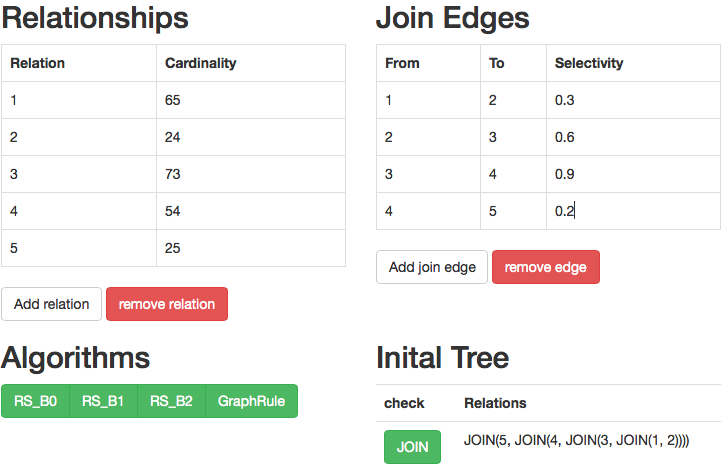
\includegraphics[width=\textwidth]{05_ResultsEvaluation/00_media/Test1.png}
  \caption{Konfiguration: Test 1}
  \label{Konfiguration:Test1}
\end{figure}

Zu diesem Zweck wurde eine Konfiguration mit fünf Relationen gewählt, die wie in Abbildung \ref{Konfiguration:Test1} zu sehen mit einander verknüpft sind.

Um festzustellen, ob alle Algorithmen für diesen speziellen Fall korrekt funktionieren, wurden zuerst alle erzeugten Pläne ausgegeben und verglichen. In einem zweiten Schritt wurden alle Äquivalenzklassen betrachtet und auf ihren Inhalt manuell geprüft.



\begin{table}[h]
\centering

\begin{tabular}{|l|l|l|l|}
\hline
                         & \multicolumn{3}{c|}{{\bf Result}} \\ \hline
{\bf Algorithmus}        & RS-B0     & RS-B1     & RS-B2     \\ \hline
{\bf Anzahl Bäume}       & 224       & 224       & 224       \\ \hline
{\bf Dauer}              & 21947086  & 20535481  & 17939373  \\ \hline
\end{tabular}

\caption{Resultat: Test 1}
\label{Result:Test1}
\end{table}

Wie in Tabelle \ref{Resultat:Test1} zu sehen ist, wurden je 224 unterschiedliche Bäume erzeugt. Eine Prüfung ergab, dass die Pläne, die durch die drei Regelmengen erzeugt wurden, alle gleich sind.

In einem nächsten Schritt wurden die Äuqivalenzklassen auf ihren Inhalt geprüft. In der obersten Äquivalenzklasse fanden sich die folgenden Planknoten:

\begin{itemize}
\item join(1,2345)
\item join(12,345)
\item join(123,45)
\item join(1234,5)
\item join(2345,1)
\item join(345,12)
\item join(45,123)
\item join(5,1234)
\end{itemize}

Bei diesen Planknoten handelt es sich um alle möglichen Permutationen der Äquivalenzklasse, die die Relationen 1 bis 5 repräsentiert. Auch alle anderen 34 Äquivalenzklassen wurden manuell geprüft. Das Ergebnis ist klar: Alle Permutationen wurden generiert und somit alle Pläne gefunden.

Es lässt sich also feststellen, dass alle Regelmengen in Bezug auf linkstiefe, azyklische Query Graphen mit 5 Relationen vollständig sind.

\subsection{Prüfung von azyklischen, sternförmigen Anfragen}

In einem zweiten Schritt wurde die Aussage von \cite{shanbhag2014optimizing} als Grundlage genommen, der behauptete, dass sternförmige Join-Trees zu umvollständigen Resultaten führen würden.

Hypothese 2: Auf Basis eines azyklischen, sternförmigen Join-Trees lässt sich mit RS-B2 der Suchraum nicht vollständig erforschen.

\begin{figure}[ht]
  \centering
  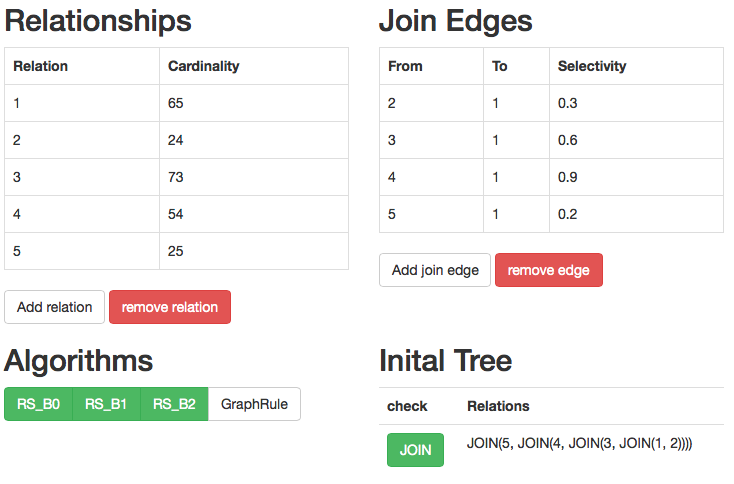
\includegraphics[width=\textwidth]{05_ResultsEvaluation/00_media/Test2.png}
  \caption{Konfiguration: Test 2}
  \label{Konfiguration:Test2}
\end{figure}


Um die Hypothese zu untersuchen wurde eine Konfiguration gewählt, die der aus Test 1 gleicht. Einziger Unterschied sind andere Join Kanten. Wie in  Abb. \ref{Konfiguration:Test2} zu sehen, sind hier alle Knoten per Join mit Knoten 5 verbunden. Es ergibt sich eine Sternform.

Nach den vorhergehenden Tests von \cite{shanbhag2014optimizing} wurde erwartet, dass durch RS-B2 nicht alle Pläne gefunden werden würden. Wie in Tabelle \ref{Result:Test2} zu sehen ist, wurde jedoch genau gleich viele Pläne mit Hilfe RS-B2 wie mit RS-B1 gefunden. 

\begin{table}[h]
\centering

\begin{tabular}{|l|l|l|l|}
\hline
                         & \multicolumn{3}{c|}{{\bf Result}} \\ \hline
{\bf Algorithmus}        & RS-B0     & RS-B1     & RS-B2     \\ \hline
{\bf Anzahl Bäume}       & 384       & 384       & 384       \\ \hline
{\bf Dauer}              & 52420049  & 49732772  & 43895234  \\ \hline
\end{tabular}

\caption{Resultat: Test 2}
\label{Result:Test2}
\end{table}


Auch die Pläne aus Test 2 wurden verglichen. Pro Regelmenge wurden die gleichen Pläne generiert. Alle 43 Äquivalenzklassen wurden geprüft und ihre Vollständigkeit festgestellt.

\begin{figure}[ht]
  \centering
  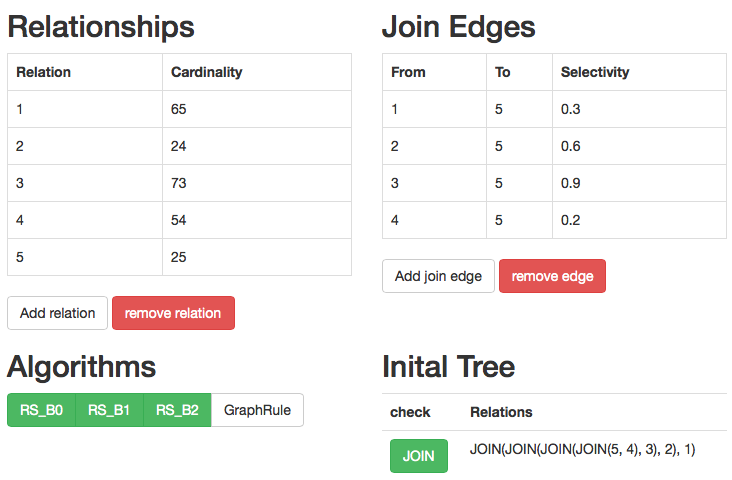
\includegraphics[width=\textwidth]{05_ResultsEvaluation/00_media/Test3.png}
  \caption{Konfiguration: Test 3}
  \label{Konfiguration:Test3}
\end{figure}


Um Sicherzustellen, dass die Aussage von \cite{shanbhag2014optimizing} nicht abhängig von der Form des Baums ist, wurde ein weiterer Test durchgeführt. Dieses mal wurde ein recht-tiefer Baum gewählt. Die Konfiguration (vgl. Abb. \ref{Konfiguration:Test3}) gleicht der vorhergehend, ausschließlich die Join-Reihenfolge wurde verändert.

\begin{table}[h]
\centering
\begin{tabular}{|l|l|l|l|}
\hline
                         & \multicolumn{3}{c|}{{\bf Result}} \\ \hline
{\bf Algorithmus}        & RS-B0     & RS-B1     & RS-B2     \\ \hline
{\bf Anzahl Bäume}       & 384       & 384       & 384       \\ \hline
{\bf Dauer}              & 53115341  & 49566404  & 44812378  \\ \hline
\end{tabular}

\caption{Resultat: Test 3}
\label{Result:Test3}
\end{table}


Wie schon im vorhergehenden Test wurden alle Pläne geprüft. Es wurden gleich viele und die gleichen Pläne wie im vorhergehenden Falle ausgegeben. Daher kann davon ausgegangen werden, dass bei einer Menge von 5 Relationen es nicht entscheidend für die Vollständigkeit ist, ob es sich initial um einen linkstiefen oder einen rechttiefen Baum gehandelt hat.



\subsection{RS-B2 ist unvollständig bei zyklischen Graphen}
Um dennoch Unvollständigkeit zu finden, wurde eine neue Hypothese aufgestellt:

Hypothese 3: RS-B2 ist bei azyklischen Join Graphen unvollständig.

Um diese Hypothese zu prüfen wurde Test 3 herangezogen und eine neue Join-Kante zwischen 3 und 4 eingezogen (vgl. Abb. \ref{Konfiguration:Test3}. Durch diese zusätzliche Kante ist eine zyklischer Join-Graph entstanden. 


\begin{figure}[ht]
  \centering
  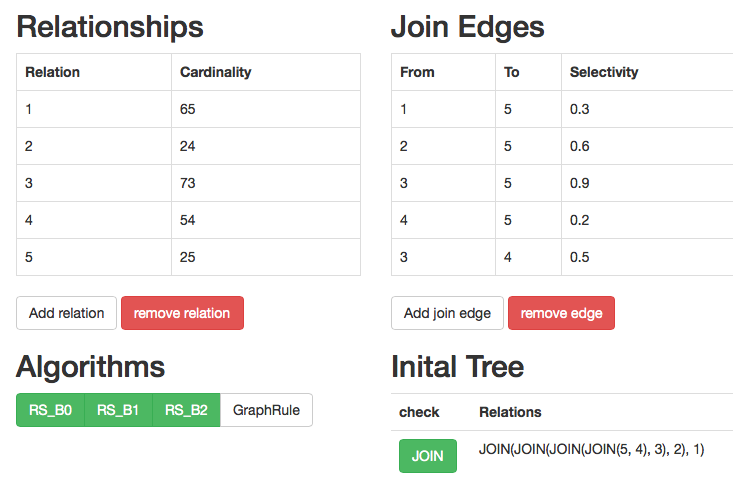
\includegraphics[width=\textwidth]{05_ResultsEvaluation/00_media/Test4.png}
  \caption{Konfiguration: Test 4}
  \label{Konfiguration:Test4}
\end{figure}

Wie erwartet wurden weniger (ca. 50\%) Pläne gefunden (vgl. Tabelle \ref{Result:Test4}). Bei einem Vergleich fiel auf, dass gerade entlang der zyklischen-Join-Kanten weniger Pläne generiert wurden.


\begin{table}[h]
\centering
\begin{tabular}{|l|l|l|l|}
\hline
                         & \multicolumn{3}{c|}{{\bf Result}} \\ \hline
{\bf Algorithmus}        & RS-B0     & RS-B1     & RS-B2     \\ \hline
{\bf Anzahl Bäume}       & 480       & 480       & 272       \\ \hline
{\bf Dauer}              & 60197027  & 56166774  & 28628930  \\ \hline
\end{tabular}

\caption{Resultat: Test 4}
\label{Result:Test4}
\end{table}

Es zeigt sich mit diesem Experiment, dass RS-B2 nicht geeignet sind, um alle Pläne für einen zyklischen Join-Graphen zu erzeugen.

\subsection{RS-B2 ist Vollständig für bestimmte zyklische Join-Graphen}










\subsection{Implementierung von Pyro(J)}
\label{sec:pyroJ}
PyroJ ist der Optimierer, der von \cite{shanbhag2014optimizing} für die Prüfung der Vollständigkeit von Pellenkofts Regelmenge RS-B2 genutzt wurde. Dies wird im folgenden Kapitel genauer beschrieben. Ebenfalls wurde auf Basis dieses Optimierers die neue Regelmenge RS-Graph implementiert und getestet. 
PyroJ basiert auf dem von \cite{roy2001multi} in C++ Implementierten Optimierer Pyro und wurde automatisch von C++ nach Java übersetzt. Der Optimierer Pyro wurde nach dem Vorbild des Volcano Optimierers entwickelt. Volcano wurde als Vorbild gewählt, da es sich bei Volcano um einen hoch-respektierten, state-of-the-art, regelbasierten Optimierer handelt, der auch die Basis von kommerziellen Datenbanksytemen wie MS SQL Server ist. Gerade die Erweiterbarkeit im Hinblick auf das Datenmodell, Executionmodell und die Möglichkeit Transformationsregeln und Operatoren hinzuzufügen, sollten übernommen werden.


Einige Unterschiede zwischen Volcano und Pyro bestehen jedoch aus Sicht von \cite{roy2001multi}:

\subsubsection{Trennung zwischen logischem und physischen Planspace}

Pyro generiert zuerst logische Pläne, die dann in physische Pläne umgesetzt werden und aus denen in einem dritten Schritt der optimale Plan ausgewählt werden kann. Diese Schritte werden nacheinander unabhängig ausgeführt. In der Realität können diese drei Schritte überlappen. So ist es möglich, dass zuerst für einen logischen Plan alle physischen Pläne erzeugt werden und dann aus diesen Plänen nur der günstigste behalten wird. Daraufhin kann dann der nächste logische Plan erzeugt werden und für ihn der günstigste physische Plan gesucht werden. Nur wenn dieser günstigste Plan billiger ist als der bisher gefundene Plan, wird der physische Plan auch weiterhin gespeichert. Dieser Ansatz kann Resourcen-schonender sein, als der in Pyro verwendete Ansatz, bei dem immer alle Daten vorgehalten werden. 

\subsubsection{Vereinigung von Äuqivalenten-Subausdrücken}

Bei Volcano ist es möglich gewesen, dass mehrere Äquivalenzklassen den selben Knoten repräsentieren. Beispielsweise kommt in der Anfrage $(A \Join B \Join C) \cup (B \Join C \Join D)$ $B$ und $C$ zweimal vor. Obwohl dies der Fall ist, werden für $B$ und für $C$ je zwei Äquivalenzklassen erzeugt. Nachdem diese beiden Relationen als unabhängig betrachtet werden, fällt auch nicht auf, dass der Ausdruck $B \Join C$ mehrfach vorkommt und somit auch in einer Äquivalenzklasse behandelt werden kann. Später wurde dieses Problem bei Volcano erkannt und mit Hilfe einer Memofunktion gelöst.

Auch Pyro(J) implementiert eine solche Memofunktion, die die Wiederverwendung von bekannten Äuqivalenzklassen erlaubt.


\subsubsection{Generierung mit Description-Files}

Ein fundamentaler Unterschied zwischen Volcano und Pyro auf den von \cite{roy2001multi} nicht hingewiesen wird, ist die Erstellung des Optimierers. Bei Pyro handelt es sich um einen fertigen Optimierer, der nicht mehr generiert werden muss. Es sind keine Description-Files vorhanden. Eine einfache Konfiguration ist nicht mehr möglich. Eine Generierung eines Optimierers findet überhaupt nicht statt.


\subsubsection{Ausführung der Experimente}

Auf PyroJ wurden von \cite{shanbhag2014optimizing} Experimente zur Überprüfung der Pellenkoft Regelmengen durchgeführt. Wie im folgenden Kapitel beschrieben, wurden Regelmengen auf ihre Vollständigkeit und Performance getestet.Außerdem  wurde eine neue Regel implementiert. 





\section{Effizienz der Regelmengen}

Um die Performance der einzelnen Regelmengen nachzuvollziehen, wurden die Regelmengen verglichen. Wie in Kapitel 4 beschrieben und unter 5.1 bemerkt, kann die Unvollständigkeit von RS-B2 (teilweise) durch den verwendeten Enumerator ExpandDAG verursacht worden sein. Daher wurde eigene Enumerator entwickelt und für die Test verwendet.

Wie im Folgenden zu sehen ist, ist der selbst implementierte Enumerator zwar sehr akkurat bei der Suche nach Planalternativen, jedoch wenig effizient. Um ein ähnliches Szenario wie in Kapitel 3 beschrieben durchführen zu können, wurde der Enumerator ExpandDAG nachimplementiert und ebenfalls in den Vergleich einbezogen.

\subsection{Vergleich des eigenen Enumerators mit ExpandDAG}


\begin{figure}[ht]
  \centering
  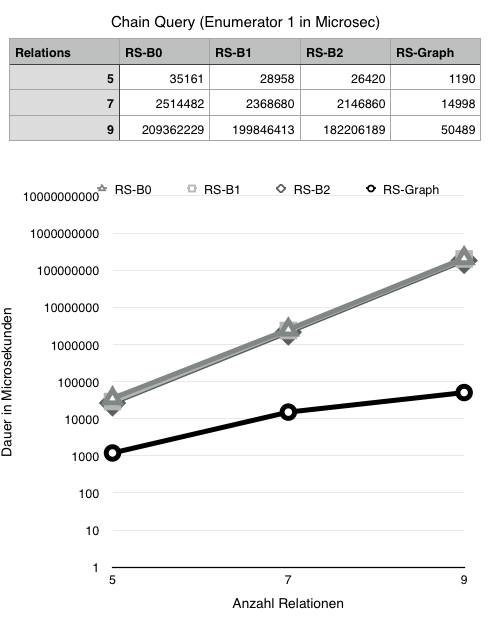
\includegraphics[width=0.5\textwidth]{05_ResultsEvaluation/00_media/ChainEnumerator1.png}
  \caption{Messergebnis des eigenen Enumerators bei kettenförmigen Anfragen}
  \label{chainQuery1}
\end{figure}

Bereits auf Abbildung \ref{chainQuery1} ist zu erkennen, wie ineffizient der Algorithmus ist. Im Vergleich der Regelmengen ist zu sehen, dass die Pellenkoft Regelmengen alle gemeinsam ähnliche Geschwindigkeiten erziehen. Jedoch ist RS-B2, der in diesem Fall vollständige Resultate generiert, der schnellste. Im Vergleich zu diesen Algorithmen ist RS-Graph erheblich schneller.


\begin{figure}[ht]
  \centering
  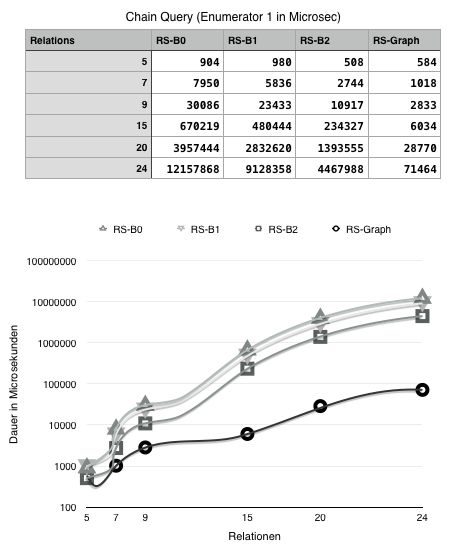
\includegraphics[width=0.5\textwidth]{05_ResultsEvaluation/00_media/ChainEnumerator2.png}
  \caption{Messergebnis des ExpandDAG bei kettenförmigen Anfragen}
  \label{chainQuery1}
\end{figure}


Mit Hilfe des zweiten Enumerators ExpandDAG wurden mehr Relationen zur Evaluation verwendet. Auch hier zeigt sich die Überlegenheit von RS-Graph.

Interessant ist insbesondere, dass im Vergleich zu den Kosten, die in Kapitel 3 zu sehen sind, RS-B2 nicht so kostenintensiv ist, wie die anderen Pellenkoft Regelmengen. Dieses Messergebnis verwundert, da in Kapitel 3 RS-B2 immer am schlechtesten abschnitt. RS-B2 schnitt dort mit exponentiellem Wachstum ab.

Das gute Abschneiden verwundert zwar im Kontext der Messungen aus Kapitel 3. Zieht man jedoch in betrachte, dass nach der Anwendung von Regeln maximal die Kommutativitätsregel ausgeführt werden kann, verringert sich die Anzahl der potenziellen Einsatzorte erheblich. Weniger Anwendungsmöglichkeiten können zu einer schnelleren Ausführung beitragen.





\subsection{Sternförmige, kreisförmige Abfragen}

Auch bei den Sternförmigen Anfragen wurde der eigene Enumerator verwendet. Wie zuvor gesehen, kann bei ExpandDAG möglicherweise nicht der vollständige Suchraum erforscht werden. Damit dieser Fehler nicht auftritt, wurde für die folgende Suche auch der eigene Enumerator eingesetzt.

Wie in Abb. \ref{starQuery123} zu sehen ist, sind die Ergebnisse ähnlich zu dem bisher gefundenen. Auch hier zeigt sich die bekannte Überlegenheit von RS-Graph. 


\begin{figure}[ht]
\centering
\begin{tabular}{|l|l|l|l|l|}
\hline
{\bf Relationen} & {\bf RS-B0} & {\bf RS-B1} & {\bf RS-B2} & {\bf RS-Graph} \\ \hline
5                & 79.381      & 75.210      & 70.986      & 913            \\ \hline
7                & 37.636.186  & 35.573.845  & 33.743.328  & 3.511          \\ \hline
\end{tabular}
  \caption{Messergebnis von sternförmigen Anfragen im eigenen Enumerator}
  \label{starQuery123}
\end{figure}


Auch bzgl. von kreisförmigen Anfragen (Abb. \ref{circle1} zeichnet sich ein ähnliches Bild. RS-Graph ist wie immer sehr performant. Die anderen Regelmengen hingegen nicht.



\begin{figure}[ht]
\centering
\begin{tabular}{|l|l|l|l|l|}
\hline
{\bf Relationen} & {\bf RS-B0} & {\bf RS-B1} & {\bf RS-B2} & {\bf RS-Graph} \\ \hline
5                & 82.395      & 79.395      & 43.331      & 1.566            \\ \hline
7                & 9.014.497  & 8.744.042  & 3.629.430  & 4.012          \\ \hline
\end{tabular}
  \caption{Messergebnis von zyklischen Anfragen im eigenen Enumerator}
  \label{circle1}
\end{figure}



\subsection{Fazit: Performance}

Wie zu erwarten war RS-Graph die effizienteste Regelmenge. Sie schnitt verglichen zu anderen Regelmengen immer besser als. Was jedoch stark verwunderlich ist, ist die Performance von RS-B2. Sie war besser als angenommen. Ebenfalls wurde festgestellt, dass die Suche nach einem Plan nicht nur abhängig von den Regelmengen, sondern auch von den Transformationsenumeratoren, die die Regeln auf die einzelnen Knoten anwenden.










